\documentclass{article}
\usepackage{geometry}
\geometry{
 a4paper,
 total={170mm,257mm},
 left=20mm,
 top=20mm,
 }
\usepackage[utf8]{inputenc}
\usepackage{graphicx}
\usepackage{kotex}
\usepackage{amsmath}
\usepackage{amssymb}
\usepackage{biblatex}
\usepackage{csquotes}
\addbibresource{citations.bib}
\title{Deliberately Injecting Poison: A Simple Method to Prevent Loops}
\author{서울대학교 전기$\cdot$정보공학부 2018-12602 이준협}
\date{}
\begin{document}
\maketitle
\section{Problem definition}

The most severe system failure that I ever had the unfortunate opportunity to experience was a Layer 2 switching loop. The reason it was caused was a dumb hub connected to two different network outlets that were connected to different workgroup switches. When the computers in the LAN sent broadcasts (e.g. ARP), the broadcasts were trapped in the network and soon the broadcasts brought down the backbone switch. As a result, our LAN was disconnected to the intranet. Similar anecdotes can readily be found on the web \cite{Anecdote2} \cite{Anecdote1}.
\begin{figure}[htb]
    \centering
    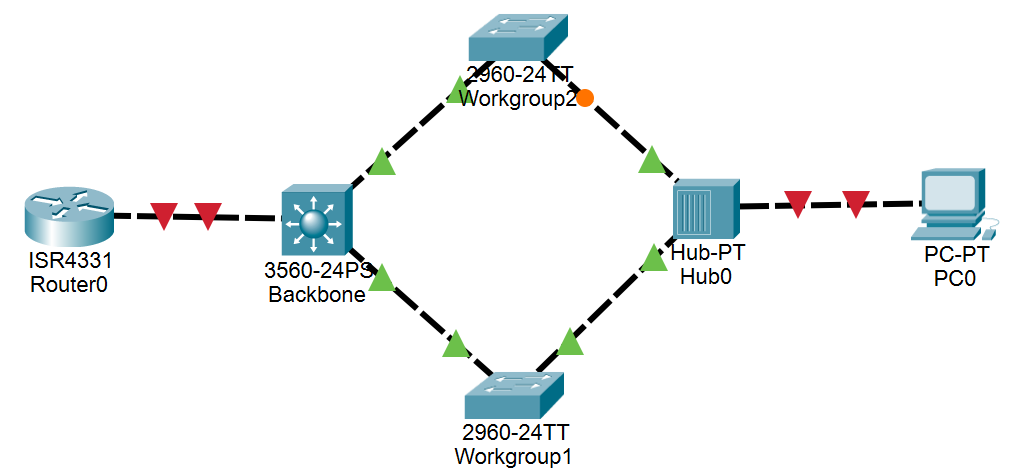
\includegraphics[scale=0.8]{storm.png}
    \caption{A simplified diagram of the offending network configuration that brought chaos.}
    \label{fig:storm}
\end{figure}

Why is this a problem? There are a couple of reasons why such a situation must be avoided at all costs.
\begin{itemize}
    \item The network failure is hard to troubleshoot because a problem at the terminal nodes causes failure of the whole network. When the whole network collapses, troubleshooting starts from the root of the network and progresses to the lowest level, which delays finding the cause of the failure. In my case, it took almost a week to find out the exact cause.
    \item The LAN that is disrupted might be part of an important network, such as the intranet of the military. Unfortunately, this was true in my case. Although the measures taken by network administrators to avoid loops are good, the rare cases that those measures fail might be critical.
\end{itemize}

Of course, theoretically loops can be prevented by the spanning tree protocol(STP) and its variants. In fact, a simple form of loop prevention called \texttt{loopback detection} was enabled on the HP switches used as the workgroup switches\cite{lbd-hp}. Also, a maximum number of mac counts was enabled on each port as to prevent malicious entities. The reason why such measures existed but failed is because of:
\begin{itemize}
    \item Human error; there are always people who are simply not proficient enough in network administration(including myself) and those people make mistakes in setting up those prevention protocols. Especially for STP, since every port in the whole network must be configured appropriately for the algorithm to work properly.
    \item Failure of the protocols; STP is known to fail when there are race conditions in choosing the root switch, for example. Moreover, when a broadcast storm occurs, many packets are dropped because of the storm and thus protocols that require periodical testing for loops do not work. This is because broadcasts with destination MAC \texttt{ffff.ffff.ffff} are unconditionally flooded.
\end{itemize}

Thus there is a need for a method that detects loops reliably and rapidly before the system is brought down.

\section{Sketch of the proposed solution}

To state the conclusion first, the proposed solution is very simple. We send a "poisonous" packet from an access port each time when a new MAC is learnt. We ensure that packet is transmitted by polling or by incorporating a bit pattern specific to the packet. When such a packet is detected, the packet is echoed and the port is shut down. The system design principle applied to this proposal is \textbf{optimize for the common case} and \textbf{separate mechanism from policy}. This method will be proven to detect a loop reliably and rapidly.

\subsection{Basic facts}

Before going into the details, some basic facts about the L2 switches that will be made use of must be noted.

\begin{itemize}
    \item The ports in the switches are divided into \textit{uplink ports} which are connected to other network equipment such as the backbone switch and \textit{access ports} which are connected to end devices.
    \item Frames sent from access ports are propagated to every devices physically connected to that port. If there is a path, the frame \textit{will} be received.
    \item The source MAC address is \textit{always} the sender of the frame, and the destination MAC address may be a valid MAC address(unicast), a range of MAC addresses(multicast), or \texttt{ffff.ffff.ffff}(broadcast).
    \item Based on the source MAC address of the frames that are sent to the access port, the access port learns the MAC addresses of the end devices. This table of learnt MAC addresses decides what frames will be forwarded to which port. For communication, the MAC address \text{must} be learnt on some port.
\end{itemize}

\subsection{Situations when loops occur}

To sense a loop, one must first analyze the common situation for a loop to occur and figure out why the existing protocols might fail.
\begin{itemize}
    \item Networks are set up to prevent failures, and connections between network equipment, such as switches, are rarely changed. This is because the equipment are usually protected physically behind locks, which can only be accessed by the network administrators.
    \item Therefore, loops \textit{usually} occur when ports connected to end devices such as PCs are interconnected. Ethernet cables are usually extended far from the wall outlets, and dumb hubs are used to extend the limited number of ports. Even with labels, it is so easy for a user with little networking knowledge to make dangerous connections.
    \item This means that at least one new connection made to an \textit{access port} causes the loop.
\end{itemize}

The telltale signal of a broadcast storm brewing in the distance is a MAC address alternating between two different ports. This is called MAC flapping. The fundamental reason why such a symptom occurs is because:

\begin{itemize}
    \item A packet sent from a network device may never return to its origin. Whether in a dumb hub or a switch, a broadcast is flooded to every port \textit{except} for the port it was received.
    \item A packet sent to an end device can never end up in another network equipment, since one end device cannot be connected to two network equipment. Packets sent to an end device ends up in a network equipment \textit{if and only if} there is a loop involving that device.
\end{itemize}

The reason why existing algorithms fail is because there is some delay between the formation of the loop and the decision to shut down the offending interfaces.
\begin{itemize}
    \item The spanning tree protocol waits until the network entities agree upon a converged view of the network topology. Worse, there might be race conditions on deciding who is the root bridge.
    \item The loopback detection method sends out loop detection packets at a fixed rate, regardless of when the loop might occur. Moreover, the detection occurs when a switch encounters a self-originated packet, thus it means that it waits until at least one packet makes a full loop.
\end{itemize}

To sum up, we are in need of a mechanism which detects loops \textit{when} the new connection to the access port is made \textit{before} a packet can make a full loop through the network. Such a detection is made by noting what kind of packets are \textit{forbidden} to be received under an acyclic topology. If this is possible, troubleshooting will be made easy because exactly the two ports who made the loop will be punished, and the network will not be frozen because the number of looping packets will be minimized.

\subsection{Description of the solution}

As can be deduced from the above description of the typical situation for loops, the policy is simple. When a \textbf{new connection} is made, a trigger for a \textbf{forbidden} event is sent to the connected device, and when it is triggered, the connections to the new device are cut off.

Translating the above conditions to the existing mechanism for L2 packet switching, we have:
\begin{itemize}
    \item New connection: When a new MAC is learnt on an access port
    \item Forbidden event: A packet from an access port is sensed on another access port.
    \item Connection is cut off: The port is put into the \texttt{shutdown} state.
\end{itemize}

There is still one point to address: how can the "packet from an access port" be known? The idea is simple: the source address for that packet must be an invalid address, like \texttt{ffff.ffff.ffff}. One can think of it as mapping the invalid source address to the address set of access ports. Then the final version of the proposal is as such:
\begin{enumerate}
    \item When a new MAC \texttt{m} is learnt on an access port, send a frame to \texttt{m} with source address \texttt{ffff.ffff.ffff} and destination address \texttt{m}.
    \item If there is no loop, the frame will be discarded, since it is an ill-formed address. However, if it is propagated into another access port, since the source address is mapped to a forbidden address, it triggers a trap.
    \item The trap echos the frame back across the link as to trigger the trap in the port that sent the frame, and shuts down the port. It then notifies the network administrator that the offending MAC \texttt{m} caused a loop.
\end{enumerate}

\subsection{Evaluation of the solution}

There are two things we must first check for \textit{reliability}.

\begin{enumerate}
    \item Can it detect a loop given the physical connection of two access ports? The answer is yes, since the creation of a loop causes the MACs that were originally accessed only through the uplink port to be newly learnt on the access port. Then the first step kicks in, and since the physical link will definitely transfer the frame to the other side, the trap will be triggered.
    \item Can a non-looping configuration cause the protocol to be triggered? No, since a frame sent from an access port must be transmitted only to the end devices by definition.
\end{enumerate}

Also, there are two things we must check for \textit{rapidity}.

\begin{enumerate}
    \item Can it detect the loop before a packet loops twice? Yes, if there existed a packet that went through the loop, it must have passed through the offending connection. Pick the first such packet(note that it might not be from a device directly connected to the port). Before the new connection, the packet must have passed through the uplink, so it will trigger the MAC to be newly learnt and the mechanism will start working. Then the port will be blocked before the packet loops again.
    \item Can it detect exactly where the new connection was made? Yes, since the solution blocks two access ports. The rest of the loop cannot be connected with access ports, since if there was such a connection, there would've been a loop in the first place (which would've been blocked). Thus it blocks exactly the new connection between access ports.
\end{enumerate}

Injecting "poison" deliberately is not a foreign concept. The whole idea of loopback detection depends on the existence of a loop protocol that shuts down connection upon detection\cite{lbd-cisco}. Compared with loopback detection, this solution improves upon it, since it does not poll and it does not wait for the packet to return to its origin.

The extra cost to pay for the solution is \textbf{one} extra transfer \textbf{per new end device connection}. Since the network topology does not change that often compared to regular broadcasts, which flood the network all the time, this seems reasonable. Also, the cost for detection is \textbf{one} bitwise NOT operation \textbf{per transmission}, since the source address is \texttt{ffff.ffff.ffff}. Compared with the cost of MAC table lookup, this also seems reasonable. These costs scale well with the increase of the LAN size, since the number of new connections/transmissions scale in ratio with the original cost of MAC learning/table lookup.

This solution utilized \textbf{optimize for the common case}, since the common cause for L2 loops is connection between access ports. Also, it utilized \textbf{separate mechanism from policy}, since it implemented the new policy for loop detection using the originally existing mechanism for transmission.

\printbibliography
\end{document}